\section{Results}
\label{sec:results}

\subsection{Sensory Modality Is Decodable from Hidden States}
\label{sec:results-probing}

Linear probes decode the dominant sensory modality far above the 16.7\% chance level across all conditions (\tabref{tab:probe_accuracy}). The implicit condition achieves \textbf{90.0\%} peak accuracy at layer 3, confirming that LLMs activate sensory representations even when the surrounding text contains no sensory language. The explicit condition reaches 92.7\%, only marginally higher. Even the control condition---where sentences use neutral framing like ``The thunder was listed in the official document''---achieves 72.0\%, indicating that the word itself carries substantial sensory signal. A permutation test on the combined condition (layer 28) confirms significance: real accuracy $= 0.904$, permutation mean $= 0.167 \pm 0.019$, $p = 0.005$.

\begin{table}[t]
\centering
\caption{Peak linear probe accuracy for 6-way sensory modality classification across conditions. Chance level is 16.7\%. All conditions substantially exceed chance, with implicit performance approaching explicit.}
\label{tab:probe_accuracy}
\begin{tabular}{@{}lccc@{}}
\toprule
\textbf{Condition} & \textbf{Best Layer} & \textbf{Peak Accuracy} & \textbf{$\times$ Chance} \\
\midrule
Implicit & 3 & {\bf 0.900} & 5.4$\times$ \\
Explicit & 3 & {\bf 0.927} & 5.6$\times$ \\
Control & 28 & 0.720 & 4.3$\times$ \\
All combined & 28 & {\bf 0.904} & 5.4$\times$ \\
\bottomrule
\end{tabular}
\end{table}

\para{Per-sense performance.}
\tabref{tab:per_sense} shows per-sense classification performance. Interoception achieves the highest F1 (0.97 combined, 0.93 implicit), likely because interoceptive words (\eg ``headache,'' ``nausea'') have few cross-modal associations. Olfaction has the lowest recall (0.76), consistent with the real-world overlap between smell and taste. In the implicit condition, auditory words are classified with 0.96 F1, reflecting the strong and distinctive linguistic contexts in which auditory objects appear.

\begin{table}[t]
\centering
\caption{Per-sense classification performance (precision / recall / F1) for the combined condition (layer 28) and implicit-only condition (layer 28). Interoception is the most distinctive; olfaction shows the most confusion with other modalities.}
\label{tab:per_sense}
\small
\begin{tabular}{@{}lcccccc@{}}
\toprule
& \multicolumn{3}{c}{\textbf{All Combined}} & \multicolumn{3}{c}{\textbf{Implicit Only}} \\
\cmidrule(lr){2-4} \cmidrule(lr){5-7}
\textbf{Sense} & \textbf{Prec.} & \textbf{Rec.} & \textbf{F1} & \textbf{Prec.} & \textbf{Rec.} & \textbf{F1} \\
\midrule
Auditory & 0.90 & 0.95 & 0.92 & 0.96 & 0.96 & {\bf 0.96} \\
Gustatory & 0.86 & 0.92 & 0.89 & 0.95 & 0.72 & 0.82 \\
Haptic & 0.90 & 0.93 & 0.92 & 0.79 & 0.88 & 0.83 \\
Interoceptive & 0.99 & 0.96 & {\bf 0.97} & 0.86 & 1.00 & {\bf 0.93} \\
Olfactory & 0.90 & 0.76 & 0.83 & 0.83 & 0.76 & 0.79 \\
Visual & 0.88 & 0.91 & 0.89 & 0.85 & 0.88 & 0.86 \\
\bottomrule
\end{tabular}
\end{table}

\subsection{Implicit and Explicit Conditions Activate Overlapping Representations}
\label{sec:results-similarity}

\figref{fig:similarity} shows that implicit and explicit conditions produce highly similar hidden states. The mean cosine similarity between implicit and explicit representations is $0.822$, significantly higher than between implicit and control ($0.767$; paired $t$-test: $t = 10.63$, $p = 6.1 \times 10^{-20}$). The explicit--control similarity ($0.763$) is comparable to implicit--control, confirming that the implicit condition activates representations closer to explicit sensory description than to neutral framing. This supports our central claim: sensory activation is spontaneous, not contingent on explicit sensory language.

\begin{figure}[t]
    \centering
    \begin{subfigure}[b]{0.48\textwidth}
        \centering
        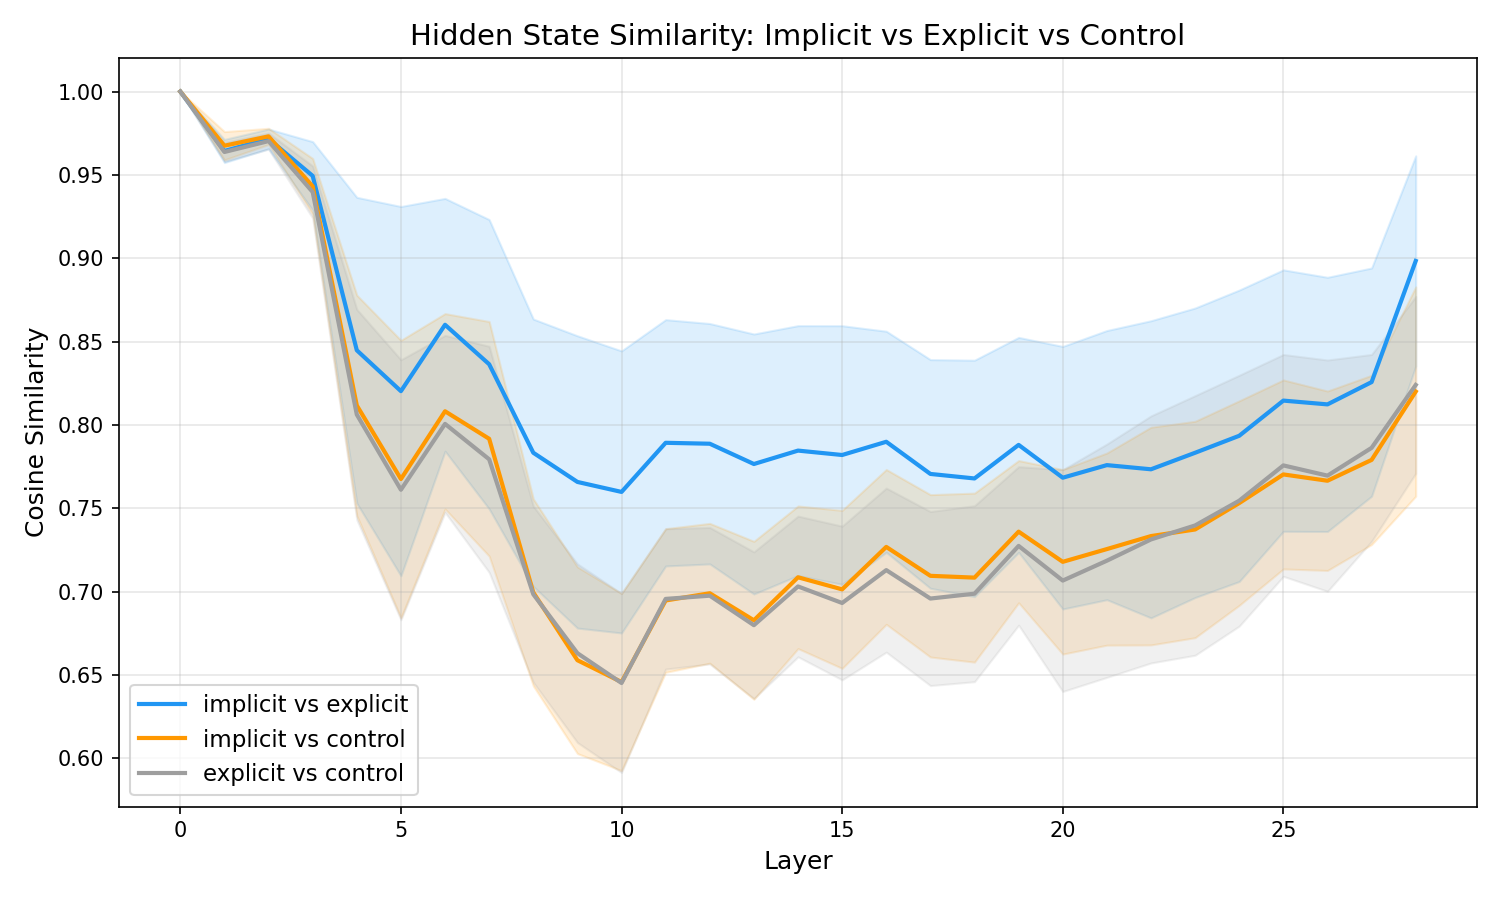
\includegraphics[width=\linewidth]{figures/implicit_vs_explicit_similarity.png}
        \caption{Cosine similarity between conditions across layers. Implicit--explicit similarity (blue) consistently exceeds implicit--control (orange).}
        \label{fig:similarity}
    \end{subfigure}
    \hfill
    \begin{subfigure}[b]{0.48\textwidth}
        \centering
        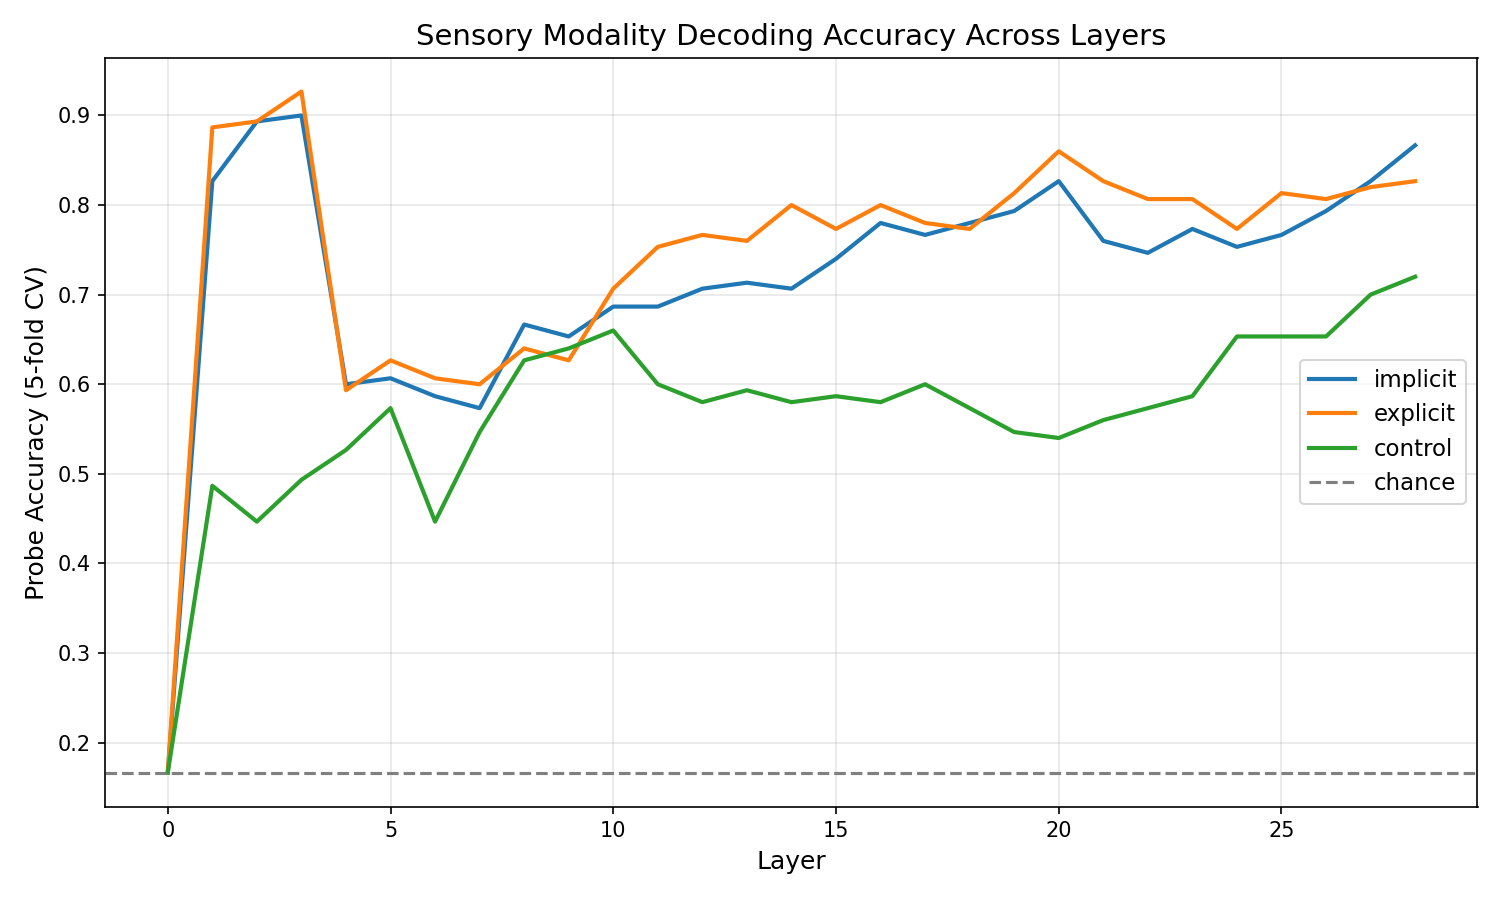
\includegraphics[width=\linewidth]{figures/layer_accuracy_curves.png}
        \caption{Probe accuracy across layers by condition. Implicit and explicit conditions achieve high accuracy early; control peaks in later layers.}
        \label{fig:overview}
    \end{subfigure}
    \caption{Condition comparison results. (a) Hidden state similarity between conditions reveals that implicit mentions activate representations closer to explicit sensory descriptions than to neutral controls. (b) Layer-wise probe accuracy shows early emergence of sensory encoding in implicit and explicit conditions.}
    \label{fig:condition_results}
\end{figure}

\subsection{Sensory Directions Form a Structured Geometry}
\label{sec:results-geometry}

The six sensory direction vectors learned by the probe exhibit a striking geometric structure (\figref{fig:geometry}). All 15 pairwise cosine similarities are negative, ranging from $-0.150$ (gustatory--olfactory) to $-0.243$ (haptic--olfactory), with a mean of $-0.200 \pm 0.028$. This contrasts sharply with the random direction baseline of $-0.001 \pm 0.100$. The negative inter-sense correlations indicate that the six senses occupy mutually opposing directions---a simplex-like structure where activating one modality suppresses the others.

\para{Interoception participates in the sensory geometry.}
The mean cosine similarity between interoceptive and classic sense directions ($-0.189 \pm 0.016$) is comparable in magnitude to the inter-classic-sense mean ($-0.205 \pm 0.030$). Interoception is not an outlier; it participates fully in the structured sensory geometry, occupying its own opposing direction alongside the five classic senses.

\begin{figure}[t]
    \centering
    \begin{subfigure}[b]{0.48\textwidth}
        \centering
        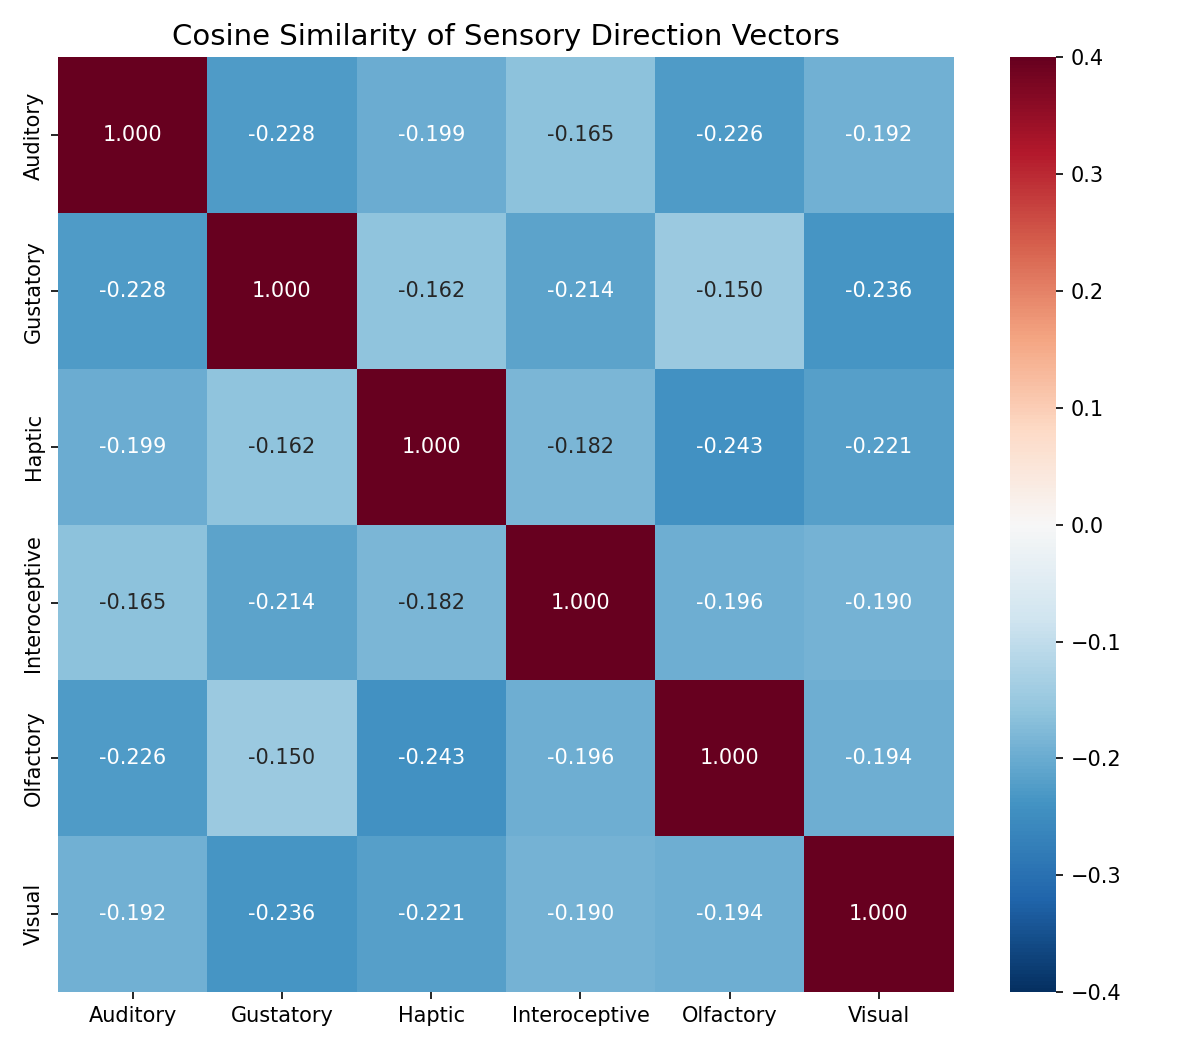
\includegraphics[width=\linewidth]{figures/sense_direction_similarity.png}
        \caption{Pairwise cosine similarity between sensory direction vectors. All off-diagonal values are negative, indicating mutually opposing directions.}
        \label{fig:heatmap}
    \end{subfigure}
    \hfill
    \begin{subfigure}[b]{0.48\textwidth}
        \centering
        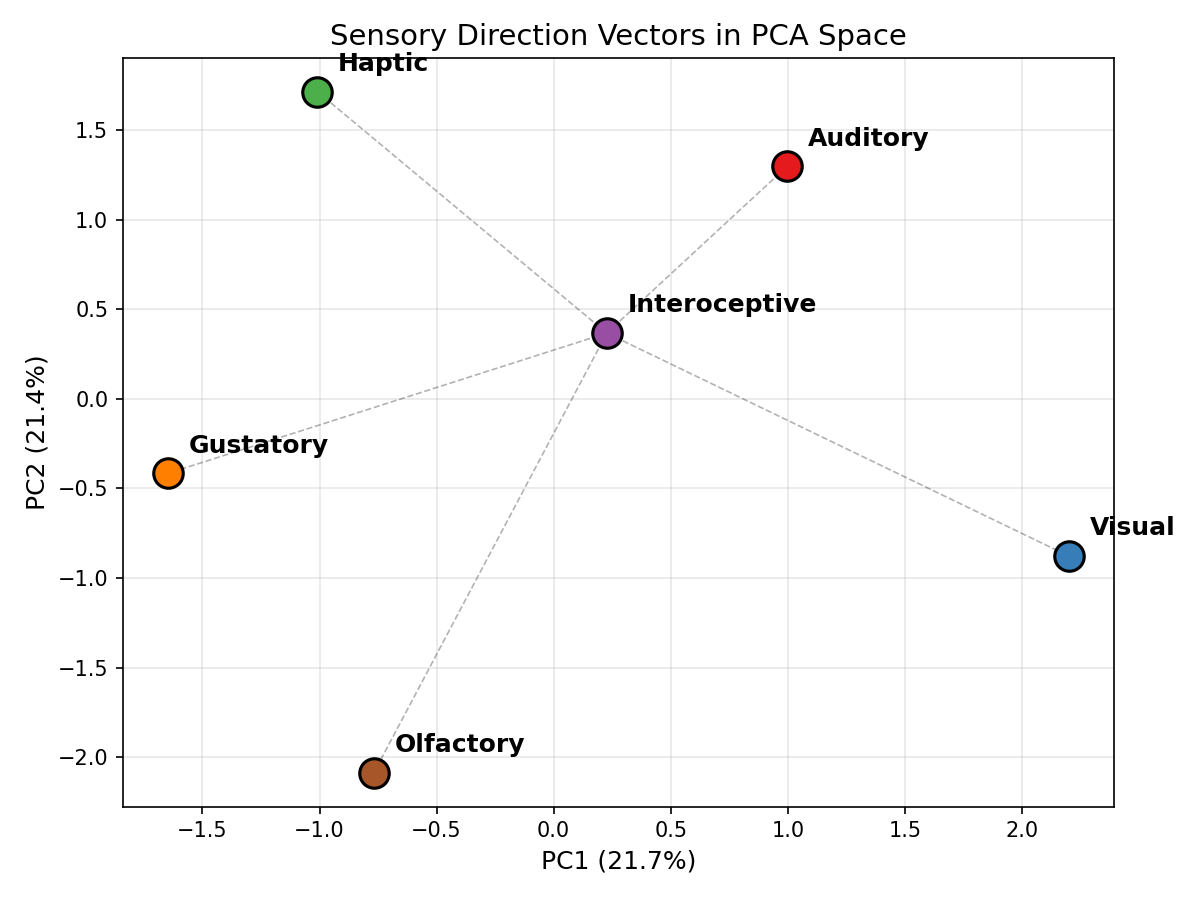
\includegraphics[width=\linewidth]{figures/sense_directions_pca.png}
        \caption{PCA projection of the six sensory direction vectors. The senses spread outward from the center, consistent with a simplex structure.}
        \label{fig:pca_directions}
    \end{subfigure}
    \caption{Geometry of the sensory subspace. (a) All pairwise similarities between sense directions are negative (mean $= -0.200$), far below the random baseline ($-0.001$). (b) PCA confirms the senses spread into distinct, approximately equidistant directions.}
    \label{fig:geometry}
\end{figure}

\subsection{Continuous Sensory Strength Is Linearly Predictable}
\label{sec:results-continuous}

Ridge regression predicts continuous Lancaster norm sensory scores with substantial accuracy (\tabref{tab:continuous}). Olfactory scores are the best predicted ($R^2 = 0.566$, Spearman $\rho = 0.726$), followed by interoceptive ($R^2 = 0.646$, $\rho = 0.480$) and gustatory ($R^2 = 0.475$, $\rho = 0.581$). All Spearman correlations are highly significant ($p < 10^{-26}$). These results show that LLM hidden states encode not just categorical sensory identity but also the graded \emph{strength} of sensory association, mirroring the continuous ratings provided by human participants.

\begin{table}[t]
\centering
\caption{Continuous sensory strength prediction from hidden states via ridge regression. $R^2$ and Spearman $\rho$ are computed against Lancaster Sensorimotor Norms human ratings. All correlations are significant at $p < 10^{-26}$.}
\label{tab:continuous}
\begin{tabular}{@{}lccc@{}}
\toprule
\textbf{Sense} & \textbf{$R^2$} & \textbf{Spearman $\rho$} & \textbf{$p$-value} \\
\midrule
Auditory & 0.438 & 0.569 & $4.95 \times 10^{-40}$ \\
Gustatory & 0.475 & 0.581 & $4.66 \times 10^{-42}$ \\
Haptic & 0.365 & 0.646 & $1.69 \times 10^{-54}$ \\
Interoceptive & {\bf 0.646} & 0.480 & $2.51 \times 10^{-27}$ \\
Olfactory & 0.566 & {\bf 0.726} & $7.76 \times 10^{-75}$ \\
Visual & 0.376 & 0.695 & $3.45 \times 10^{-66}$ \\
\bottomrule
\end{tabular}
\end{table}

\subsection{Sensory Representations Emerge Early}
\label{sec:results-emergence}

\figref{fig:emergence} shows per-sense probe accuracy across all 29 layers. All senses are decodable above $2\times$ chance by layer 1. Auditory representations are a notable exception: they achieve \emph{perfect} accuracy (1.000) at layer 0---the embedding layer---suggesting that auditory associations are encoded directly in the token embeddings before any contextual processing occurs. Other senses peak at later layers: gustatory at layer 25, haptic at layer 24, interoceptive at layer 16, olfactory at layer 9, and visual at layer 27. This staggered emergence suggests that different sensory modalities may rely on different depths of contextual processing.

\begin{figure}[t]
    \centering
    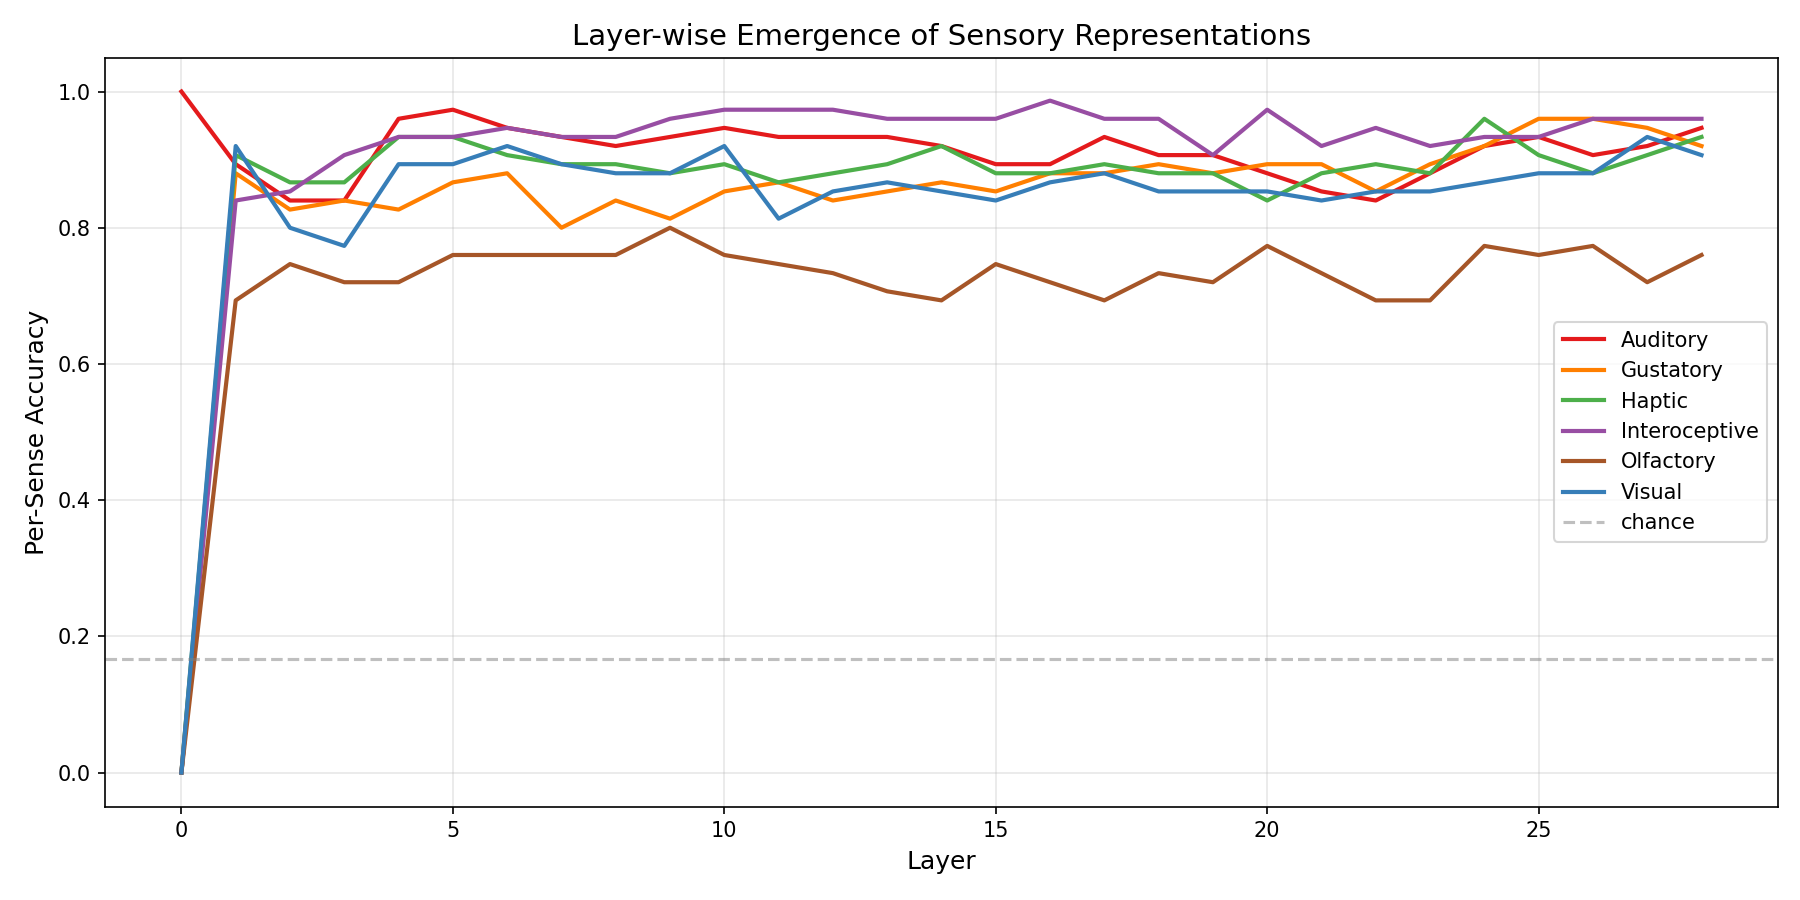
\includegraphics[width=0.7\textwidth]{figures/layerwise_per_sense.png}
    \caption{Per-sense probe accuracy across layers (all conditions combined). All senses emerge above $2\times$ chance by layer 1. Auditory is perfectly decodable at the embedding layer (layer 0); other senses peak at varying depths, suggesting modality-dependent processing requirements.}
    \label{fig:emergence}
\end{figure}
